\section{Allgemeine Anforderungen}
In diesem Abschnitt sollen allgemeine Anforderungen beschrieben werden, die für das Gesamtsystem gelten. Dazu wird ein Ablaufszenario beschrieben, dass beschreibt, wie die Akteure (Rampen und Fahrzeuge) miteinander interagieren, damit ein vollautomatisierter Warenfluss entsteht.
\subsection{Ablaufszenario}\label{AL} 
Das Ablaufszenario beschreibt die Schritte, die von den Akteuren ausgeführt werden, um das Ziel zu erreichen, aus logischer Sicht ohne dabei auf die technischen Implementierungsdetails einzugehen. Es dient als Basis für die Implementierung sowohl des physischen Systems als auch der Simulationssoftware. Abbildung \ref{Abl1} zeigt den schemenhaften Aufbau des Umschlagslagers. Die Rampen unterteilen sich in Eingangs-, Zwischenlager- und Ausgangsrampen abhängig von ihrer Position. Pakete treffen am Eingang ein und werden dort aufgenommen. 
\\\\
\begin{figure}[h!]
	\centering
		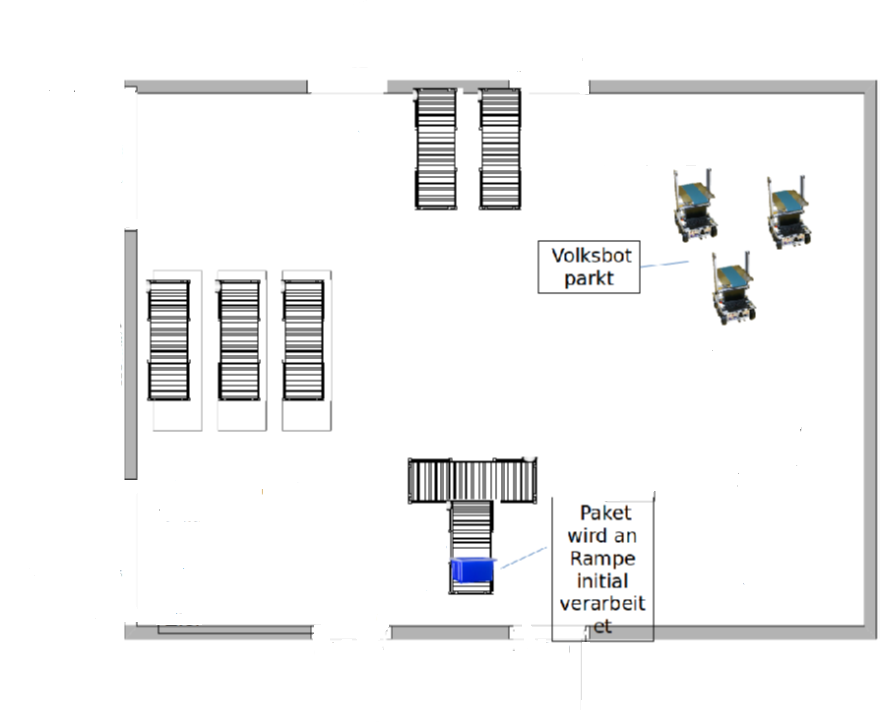
\includegraphics[width=0.6\textwidth]{Alg1}        
		\caption{Teil 1 Ablaufszenario}
	\label{Abl1}
\end{figure}
\\
Die Eingangsrampe sucht für das Paket ein Ziel, indem das Zwischenlager gefragt wird, ob Platz vorhanden ist oder ob am Ausgang Bedarf besteht. Sobald ein Ziel gefunden ist, sucht die Rampe über eine Auktion ein Transportmittel. Die Bots berechnen eine Aufwandsabschätzung und schicken diese an die Rampe, die einen Bot auswählt (Vgl.\ref{Abl2}). 
\\   
\begin{figure}[h!]
	\centering
		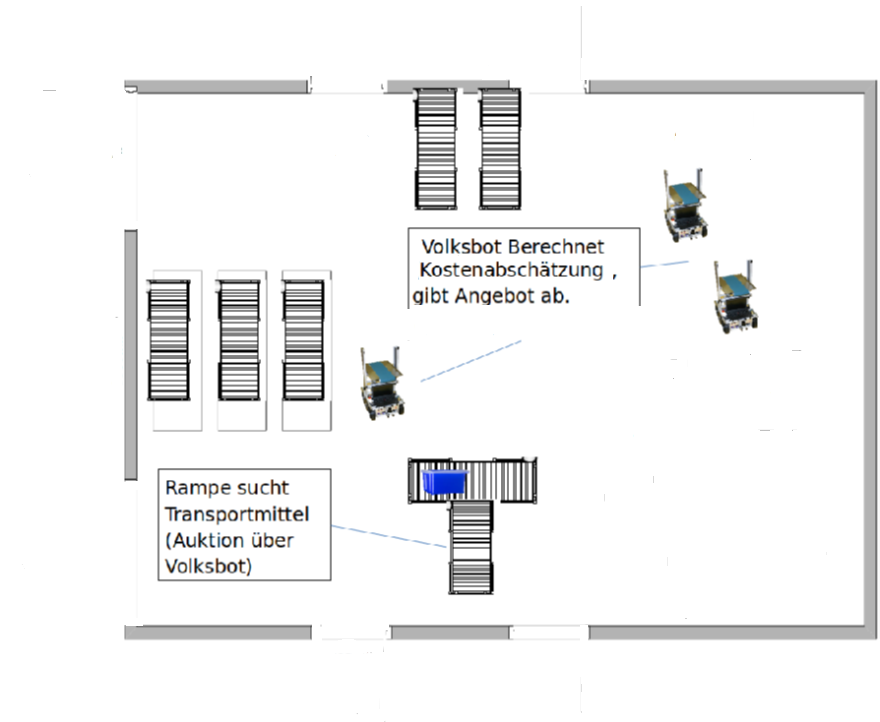
\includegraphics[width=0.6\textwidth]{Alg2}        
		\caption{Teil 2 Ablaufszenario}
	\label{Abl2}
\end{figure} 
\\
Die Bots fahren zu den Eingangsrampen, laden die Pakete auf und bringen diese zu den Zwischenrampen oder Ausgangsrampen (Vgl.\ref{Abl3}). Pakete, die im Zwischenlager ankommen, werden analog dem beschriebenen Ablaufmuster von den Bots zu den Rampen gebracht. Der einzige Unterschied besteht darin, dass die Ausgangsrampen anfragen, ob ein gewünschtes Paket im Zwischenlager vorhanden ist.
\begin{figure}[h!]
	\centering
		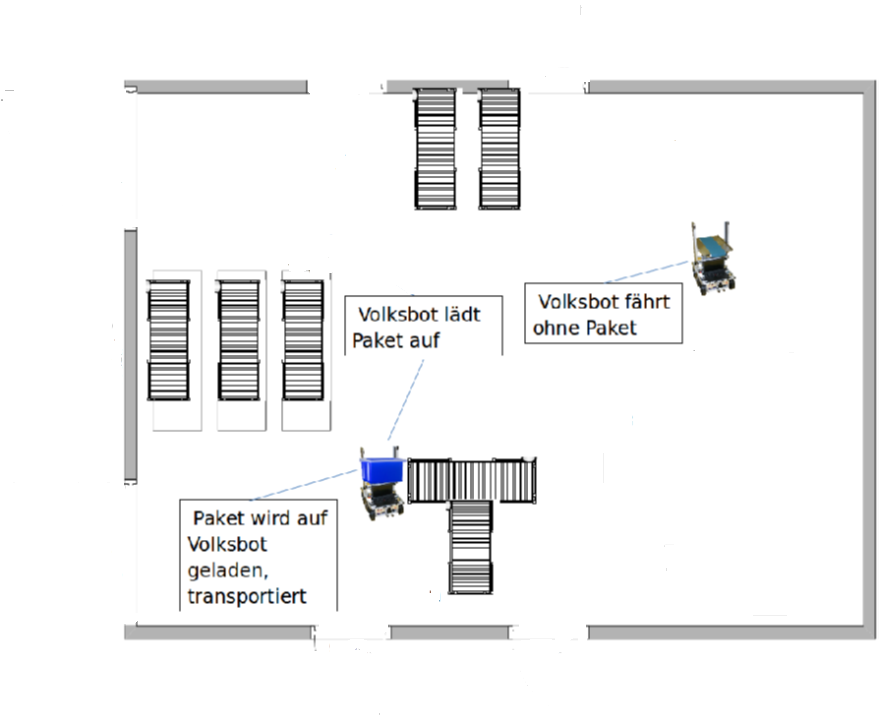
\includegraphics[width=0.6\textwidth]{Alg3}        
		\caption{Teil 3 Ablaufszenario}
	\label{Abl3}
\end{figure}  
